\documentclass{beamer}

\usetheme{Berkeley}
\usepackage{graphicx}
\graphicspath{ {./images/} }

\title{Sprint 1}

\subtitle{IO and Algorithm}

\author{Albert van Kiel, Timo Hermsen, Robin Baneke, Max van Hasselt, Robert Kleef and Menno Prinzhorn}

\date{\today}

\begin{document}

\begin{frame}
    \titlepage
\end{frame}

\section{Background}
    
\begin{frame}{Background}
    Project background
    \\~\\
    \begin{itemize}
        \item SIGPROC library
        \item eScience center
        \item Asteria
        \item IO/Algorithm
    \end{itemize}
\end{frame}

\section{Methodology}
	\begin{frame}{Methodology}
	What were our methods?     
	\begin{itemize}
		\item SCRUM
		\item Sprint reviews
	\end{itemize}
\end{frame}

\section{Goals}
\begin{frame}{Goals}
    Our goals for Asteria      
    \begin{itemize}
        \item Refactoring SIGPROC library
        \item Python/C++
        \item Tests minimal 60\% code coverage
    \end{itemize}
\end{frame}

\section{Modules}
\begin{frame}{Modules}
	These modules are present and usable in the Asteria library     
	\begin{itemize}
		\item Filterbank
		\item Clipping
		\item Dedisperse
		\item Timeseries
		\item Fourier
		\item Pipeline
		\item Plot
	\end{itemize}
\end{frame}

\section{Filterbank}
\begin{frame}{Filterbank}
	\begin{itemize}
		\item Read filterbank files
		\item Generate mock data
	\end{itemize}
\end{frame}

\section{Clipping}
\begin{frame}{Clipping}
<<<<<<< HEAD
	\begin{columns}
		\begin{column}{0.5\textwidth}
			Filter samples with noise
			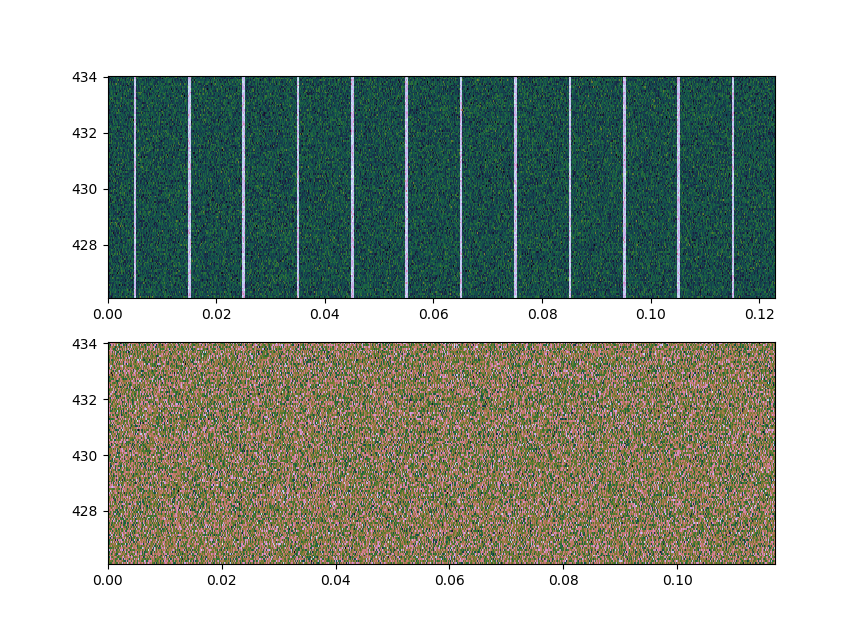
\includegraphics[width=\columnwidth]{filter_samples}
		\end{column}
		\begin{column}{0.5\textwidth}
			Filter frequencies with noise
			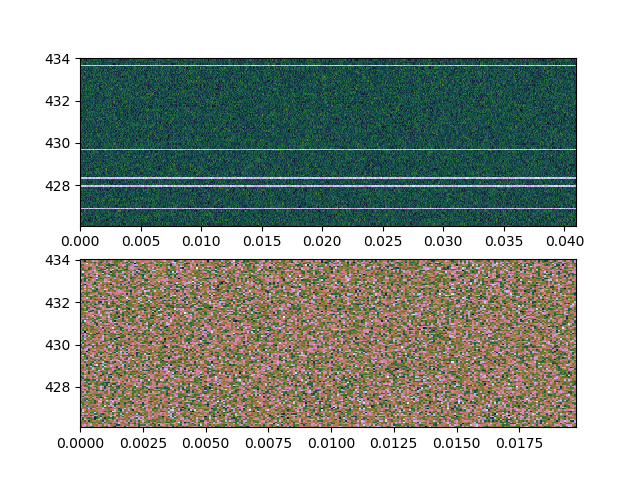
\includegraphics[width=\columnwidth]{filter_freqs}
		\end{column}
	\end{columns}
=======
	\begin{itemize}
		\item Filter samples
		\item Filter channels
	\end{itemize}
>>>>>>> ade28e3035c75d64b1029a5101c16ebdb01c9a96
\end{frame}

\section{Dedisperse}
\begin{frame}{Dedisperse}
	Dedispersion
\end{frame}

\section{Timeseries}
\begin{frame}{Timeseries}
	\begin{itemize}
		\item Downsampling
	\end{itemize}
\end{frame}

\section{Fourier}
\begin{frame}{Fourier}
	\begin{itemize}
		\item FFT Matrix
		\item Discrete Fourier Transform
		\item Cooley-Tukey
		\item Shirt zero-frequency
	\end{itemize}
\end{frame}

\section{Pipeline}
\begin{frame}{Pipeline}
	\begin{figure}
		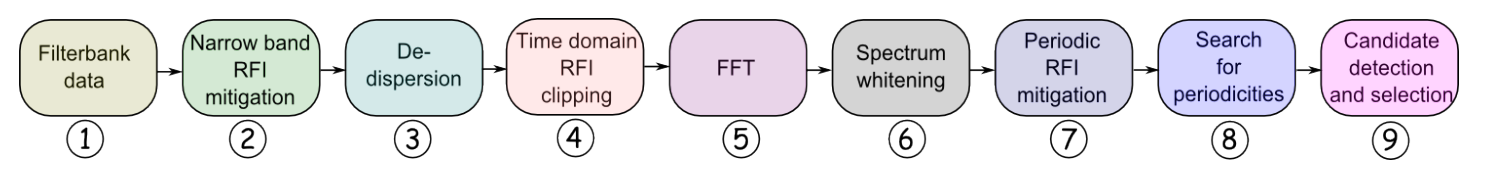
\includegraphics[width=\textwidth]{pipeline-order}
	\end{figure}
\end{frame}

\section{Plot}
\begin{frame}{Plot}
	\begin{itemize}
		\item Plot
		\item Waterfall
	\end{itemize}
\end{frame}

\section{End}
\begin{frame}{Questions?}
	Questions?
\end{frame}

\end{document}
